\chapter{\babDua}
\label{bab:2}
Pada bab ini dijlaskan secara rinci mengenai detil pekerjaan yang dilakukan oleh peserta kerja praktik selama program kerja praktik berlangsung. Latar belakang pekerjaan hingga hasil pekerjaan dijelaskan pada bab ini.

\section{Latar Belakang Pekerjaan}
\label{sec:latar-belakang}

Pelaksana kerja praktik terlibat dalam penelitian terkait manajemen klaster Kafka di Computer Systems Laboratory (CSL) Fakultas Ilmu Komputer Universitas Indonesia. Penelitian ini berfokus pada optimalisasi partisi topik untuk meningkatkan performa sistem streaming data real-time berbasis Kafka. Proyek ini merupakan bagian dari penelitian bertajuk \textit{Efficient Topic Partitioning of Apache Kafka for High-Reliability Real-Time Data Streaming Applications}. Tugas pelaksana kerja praktik adalah menjalankan eksperimen yang bertujuan untuk menguji algoritma BroMax dan BroMin, yang digunakan untuk menentukan jumlah partisi optimal dalam klaster Kafka guna memaksimalkan throughput.

\section{Deskripsi Pekerjaan}
\label{sec:deskripsi-pekerjaan}

Pelaksana kerja praktik bertanggung jawab atas konfigurasi dan pengelolaan eksperimen end-to-end. Proses dimulai dengan penyiapan VM di Google Cloud Platform (GCP) dan infrastruktur Universitas Indonesia (DGX dan BMKGCS), yang digunakan untuk menjalankan simulasi klaster Kafka. Tugas utama meliputi instalasi dependencies, pengaturan Kafka broker, serta analisis hasil eksperimen untuk mengukur performa sistem, khususnya throughput dan latensi, saat algoritma BroMax dan BroMin diterapkan.

Pekerjaan dilakukan secara hybrid dari pukul 08.00 a.m. WIB hingga pukul 12.00 p.m. WIB, dengan kehadiran di lab hanya pada hari Jumat, sedangkan hari-hari lainnya bekerja secara remote. Meskipun demikian, pekerjaan tetap mengikuti jadwal sprint yang ditetapkan dalam kerangka metodologi Scrum, memastikan target pekerjaan tercapai dalam setiap periode. Hasil eksperimen dianalisis dan dilaporkan kepada dosen pembimbing untuk evaluasi lebih lanjut.

\section{Tinjauan Pustaka}
\label{sec:tinjauan-pustaka}

Penelitian yang dilakukan selama kerja praktik ini melibatkan sejumlah konsep penting dalam pengelolaan sistem distribusi data real-time dengan menggunakan Apache Kafka dan teknologi pendukung lainnya. Konsep-konsep ini menjadi fondasi utama dalam penelitian dan pengembangan yang dilakukan.

\subsection{Apache Kafka}

Apache Kafka adalah platform open-source yang dirancang untuk menangani streaming data secara real-time dengan throughput tinggi dan latensi rendah. Kafka memungkinkan integrasi data yang cepat dan efisien melalui model distribusi data yang skalabel. Dalam sistem ini, data dibagi menjadi topik-topik yang dipartisi, sehingga memungkinkan pemrosesan paralel yang lebih efisien di seluruh klaster \citep{elsevier:kafka}. Partisi pada topik Kafka sangat penting karena memungkinkan distribusi beban kerja yang merata antar broker, sehingga meningkatkan kemampuan sistem untuk menangani data dalam jumlah besar tanpa menimbulkan bottleneck \citep{elsevier:kafka}. Selain itu, dengan optimalisasi jumlah partisi yang tepat, throughput sistem dapat dimaksimalkan, sehingga menjaga kinerja tinggi meskipun volume data yang diproses sangat besar \citep{elsevier:kafka}.

\subsection{Docker Containerization}

Docker Containerization adalah teknologi yang memungkinkan aplikasi dijalankan dalam container yang terisolasi, sehingga dapat memisahkan lingkungan eksekusi aplikasi dari sistem host. Dalam konteks kerja praktik ini, Docker digunakan untuk mengelola dan menjalankan klaster Kafka pada berbagai infrastruktur, termasuk Google Cloud Platform dan sistem internal. Docker memungkinkan konsistensi lingkungan, meminimalkan konflik konfigurasi, serta meningkatkan portabilitas sistem distribusi data real-time yang digunakan selama eksperimen \citep{its:docker}. Dengan Docker, seluruh proses deployment Kafka menjadi lebih efisien karena setiap node dalam klaster dapat dijalankan dengan konfigurasi yang seragam, mengurangi kesalahan operasional dan mempercepat penyebaran aplikasi \citep{its:docker}.

\subsection{Apache Zookeeper}

Apache Zookeeper adalah layanan koordinasi terpusat yang digunakan untuk mengelola metadata dan menjaga konsistensi di dalam klaster Kafka. Zookeeper bertugas mengatur eleksi pemimpin partisi, menyinkronkan data antar broker, serta memastikan bahwa setiap perubahan dalam klaster Kafka ditangani dengan cepat dan efisien \citep{comp:zookeeper}. Dalam konteks Kafka, Zookeeper memainkan peran penting dalam memastikan bahwa sistem tetap fault-tolerant. Jika terjadi kegagalan pada salah satu broker, Zookeeper secara otomatis memilih broker lain untuk menjadi pemimpin, menjaga kestabilan sistem selama proses pemrosesan data real-time berlangsung \citep{comp:zookeeper}. Zookeeper juga menyimpan informasi konfigurasi mengenai topik dan partisi Kafka, memastikan bahwa produser dan konsumen dapat berinteraksi dengan sistem secara konsisten \citep{comp:zookeeper}.

\subsection{Distributed System}

Distributed System adalah sistem yang terdiri dari beberapa node yang terhubung dan bekerja bersama untuk mencapai tujuan tertentu. Dalam konteks Kafka, sistem terdistribusi ini memastikan bahwa data dapat diolah secara paralel dan skalabel di berbagai broker yang tersebar dalam klaster. Keunggulan dari sistem terdistribusi seperti Kafka adalah kemampuannya untuk tetap berfungsi meskipun terjadi kegagalan pada satu atau beberapa node dalam klaster \citep{ieee:distributed}. Dalam sistem terdistribusi Kafka, partisi topik didistribusikan ke berbagai broker, sehingga meningkatkan ketersediaan data dan mempercepat proses pengiriman data dari produser ke konsumen \citep{ieee:distributed}. Sistem ini juga memungkinkan replikasi data secara otomatis, di mana salinan data disimpan di beberapa broker untuk meningkatkan keandalan dan redundansi sistem \citep{ieee:distributed}.

\section{Metodologi Pekerjaan}



\section{Membuat Tabel}
\label{sec:latexTable}
Tabel pada Latex dapat dibuat dengan bantuan \textit{website} seperti \url{https://www.tablesgenerator.com/}.
Dengan menggunakan \textit{website} ini, maka pembuatan tabel akan menjadi lebih mudah.
\textit{User interface} dari \url{https://www.tablesgenerator.com/} dapat dilihat pada Gambar \ref{fig:tablesgenerator}.

\begin{figure}
	\centering
	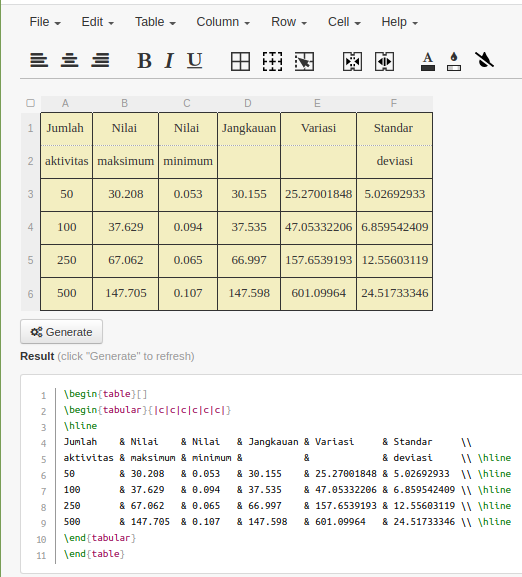
\includegraphics[width=0.5\textwidth]{assets/pics/tablesgenerator-dot-com.png}
	\caption{\textit{User interface} dari \textit{website} https://www.tablesgenerator.com/}
	\label{fig:tablesgenerator}
\end{figure}

Di sisi lain, tabel juga dapat diberi label dan caption seperti pada gambar.
Caption pada tabel terletak pada bagian atas tabel.
Contoh tabel sederhana dapat dilihat pada \tab~\ref{tab:tab1}.

\begin{table}
	\centering
	\caption{Contoh Tabel}
	\label{tab:tab1}
	\begin{tabular}{| l | c r |}
		\hline
		& kol 1 & kol 2 \\
		\hline
		baris 1 & 1 & 2 \\
		baris 2 & 3 & 4 \\
		baris 3 & 5 & 6 \\
		baris 4 & 7 & 8 \\
		baris 5 & 9 & 10 \\
		\hline
		jumlah  & 25 & 30 \\
		\hline
	\end{tabular}
\end{table}

Adapun untuk membuat tabel panjang yang bisa melebihi dari satu halaman, gunakan perintah \code{\bslash{}begin\{longtable\}} sebagai pengganti \code{\bslash{}begin\{table\}}. Di dalam \code{longtable} tidak perlu lagi ada \code{\bslash{}begin\{tabular\}}. Kemudian, tambahkan tanda \code{\bslash{}\bslash{}} setelah baris \code{\bslash{}label\{....\}}, agar tidak menimbulkan error saat menampilkan \f{caption} di bagian atas tabel. Kemudian, untuk membatasi header yang ingin diulang pada halaman-halaman berikutnya, gunakan perintah \code{\bslash{}endhead}. Contohnya adalah sebagai berikut:

\begin{longtable}{| l | c r |}
\caption{Contoh Tabel Panjang}
\label{tab:tab2} \\
\hline
& kol 1 & kol 2 \\
\hline
\caption[]{Contoh Tabel Panjang (sambungan)} \\
\hline
& kol 1 & kol 2 \\
\hline
\hline
\hline
baris 1  & 1 & 2 \\
baris 2  & 3 & 4 \\
baris 3  & 5 & 6 \\
baris 4  & 7 & 8 \\
baris 5  & 9 & 10 \\
baris 6  & 11 & 12 \\
baris 7  & 13 & 14 \\
baris 8  & 15 & 16 \\
baris 9  & 17 & 18 \\
baris 10 & 19 & 20 \\
baris 11 & 21 & 22 \\
baris 12 & 23 & 24 \\
baris 13 & 25 & 26 \\
baris 14 & 27 & 28 \\
baris 15 & 29 & 30 \\
baris 16 & 31 & 32 \\
\end{longtable}

Ada jenis tabel lain yang dapat dibuat dengan \latex~berikut beberapa diantaranya.
Contoh-contoh ini bersumber dari \url{http://en.wikibooks.org/wiki/LaTeX/Tables}

\begin{table}
	\centering
	\caption{An Example of Rows Spanning Multiple Columns}
	\label{row.spanning}
	\begin{tabular}{|l|l|*{6}{c|}}
		No & Name & \multicolumn{3}{|c|}{Week 1} & \multicolumn{3}{|c|}{Week 2} \\
		& & A & B & C & A & B & C\\
		\hline
		1 & Lala & 1 & 2 & 3 & 4 & 5 & 6\\
		2 & Lili & 1 & 2 & 3 & 4 & 5 & 6\\
		3 & Lulu & 1 & 2 & 3 & 4 & 5 & 6\\
		\hline
	\end{tabular}
\end{table}

\begin{table}
	\centering
	\caption{An Example of Columns Spanning Multiple Rows}
	\label{column.spanning}
	\begin{tabular}{|l|c|l|}
		\hline
		Percobaan & Iterasi & Waktu \\
		\hline
		Pertama & 1 & 0.1 sec \\ \hline
		\multirow{2}{*}{Kedua} & 1 & 0.1 sec \\
		& 3 & 0.15 sec \\
		\hline
		\multirow{3}{*}{Ketiga} & 1 & 0.09 sec \\
		& 2 & 0.16 sec \\
		& 3 & 0.21 sec \\
		\hline
	\end{tabular}
\end{table}

\begin{table}
	\centering
	\caption{An Example of Spanning in Both Directions Simultaneously}
	\label{mix.spanning}
	\begin{tabular}{cc|c|c|c|c|}
		\cline{3-6}
		& & \multicolumn{4}{|c|}{Title} \\ \cline{3-6}
		& & A & B & C & D \\ \hline
		\multicolumn{1}{|c|}{\multirow{2}{*}{Type}} &
		\multicolumn{1}{|c|}{X} & 1 & 2 & 3 & 4\\ \cline{2-6}
		\multicolumn{1}{|c|}{}                        &
		\multicolumn{1}{|c|}{Y} & 0.5 & 1.0 & 1.5 & 2.0\\ \cline{1-6}
		\multicolumn{1}{|c|}{\multirow{2}{*}{Resource}} &
		\multicolumn{1}{|c|}{I} & 10 & 20 & 30 & 40\\ \cline{2-6}
		\multicolumn{1}{|c|}{}                        &
		\multicolumn{1}{|c|}{J} & 5 & 10 & 15 & 20\\ \cline{1-6}
	\end{tabular}
\end{table}


\section{Keterkaitan Teori Dengan Penelitian}
\label{sec:keterkaitan}
\todo{Ada baiknya setelah menjelaskan teori-teori, Anda menjelaskan apa kaitan teori tersebut dengan penelitian Anda.
Hal ini tentunya membantu pembaca dalam memahami bahwa teori yang Anda paparkan memang penting untuk memahami penelitian Anda nantinya.}

\begin{figure}
	\centering
	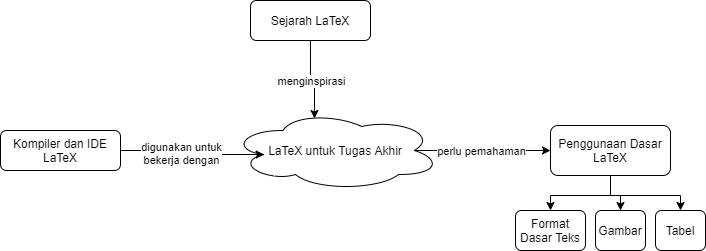
\includegraphics[width=\textwidth]{assets/pics/research_concept_map.png}
	\caption{Keterkaitan konsep hasil studi literatur terhadap penelitian}
	\label{fig:research_concept_map}
\end{figure}

\noindent\todo{
	Jelaskan \pic~\ref{fig:research_concept_map} di sini.
	Setiap gambar pada tugas akhir butuh penjelasan.
	Gambar hadir untuk mempermudah membaca memahami konteks, tetapi tidak bisa berdiri sendiri tanpa penjelasan.
	Terkait gambar, Anda juga bisa mengatur skalanya.
	Gambar kali ini lebarnya 0,8x dari lebar teks halaman.
}
